\title{Perfomancevergleich Mesh Netzwerke}

\team{%
    Raffael Anklin,
    Robin Bobst,
    Cyrill Horath}

%\client{Important Client}

\expert{%
	Jürg M. Stettbacher}

\coaches{%
    Manuel Di Cerbo,
    Matthias Meier}
    

\fssummary{
Die Vernetzung von Sensoren und Aktoren im Low-Power Bereich stellt eine grosse Herausforderung dar.
Immer öfter werden Systeme in diesem Bereich mit sogenannten \textit{Wireless Sensor Networks} realisiert.
Mit typischerweise geringen Latenzzeiten, kleinen Datenraten und kleinem Stromverbrauch eignen sich die drei bekanntesten \textit{Low-Power-Mesh-Protokolle} Bluetooth Mesh, Thread und ZigBee perfekt für solche Anwendungen.
Wo die drei Protokolle ihre Stärken und wo allenfalls Schwächen haben ist nur schwer ersichtlich.
In einem ausführlichen Performancetest unter ändernden Bedingungen werden nun Unterschiede sowie Vor- und Nachteile aufgezeigt.
}

\fsgraphics{
\centering
	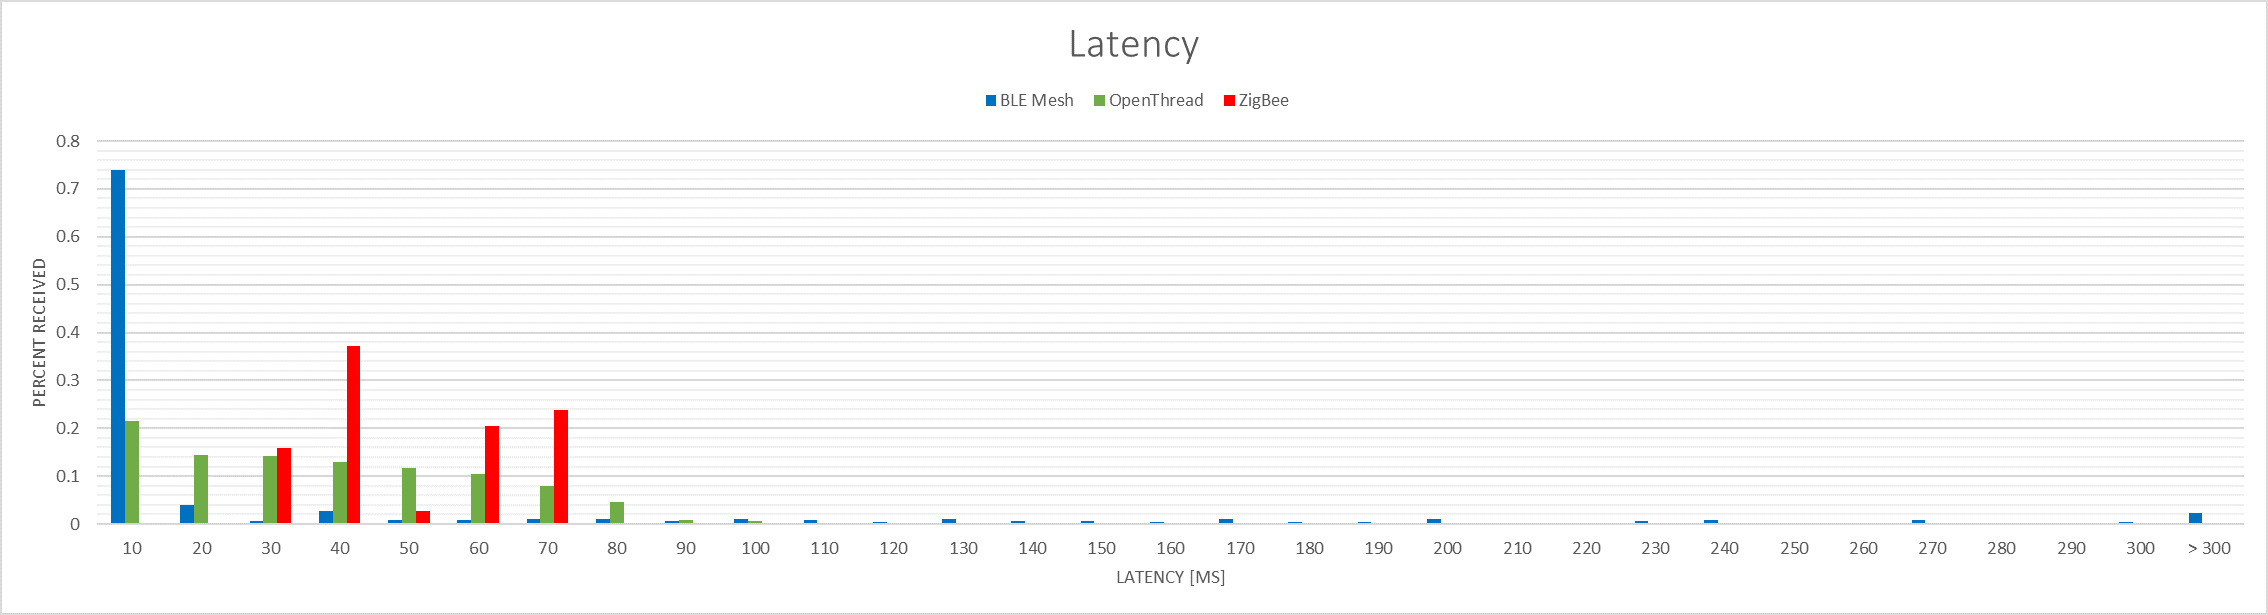
\includegraphics[width=\textwidth]{graphics/Latency_2_Wohnung.png}
    \graphicscaption{Auswertung Messergebnisse Latenzzeiten}
}

\fscontent{
    \section{Konzept}

    \newcol
    \section{Umsetzung}
    \begin{center}
    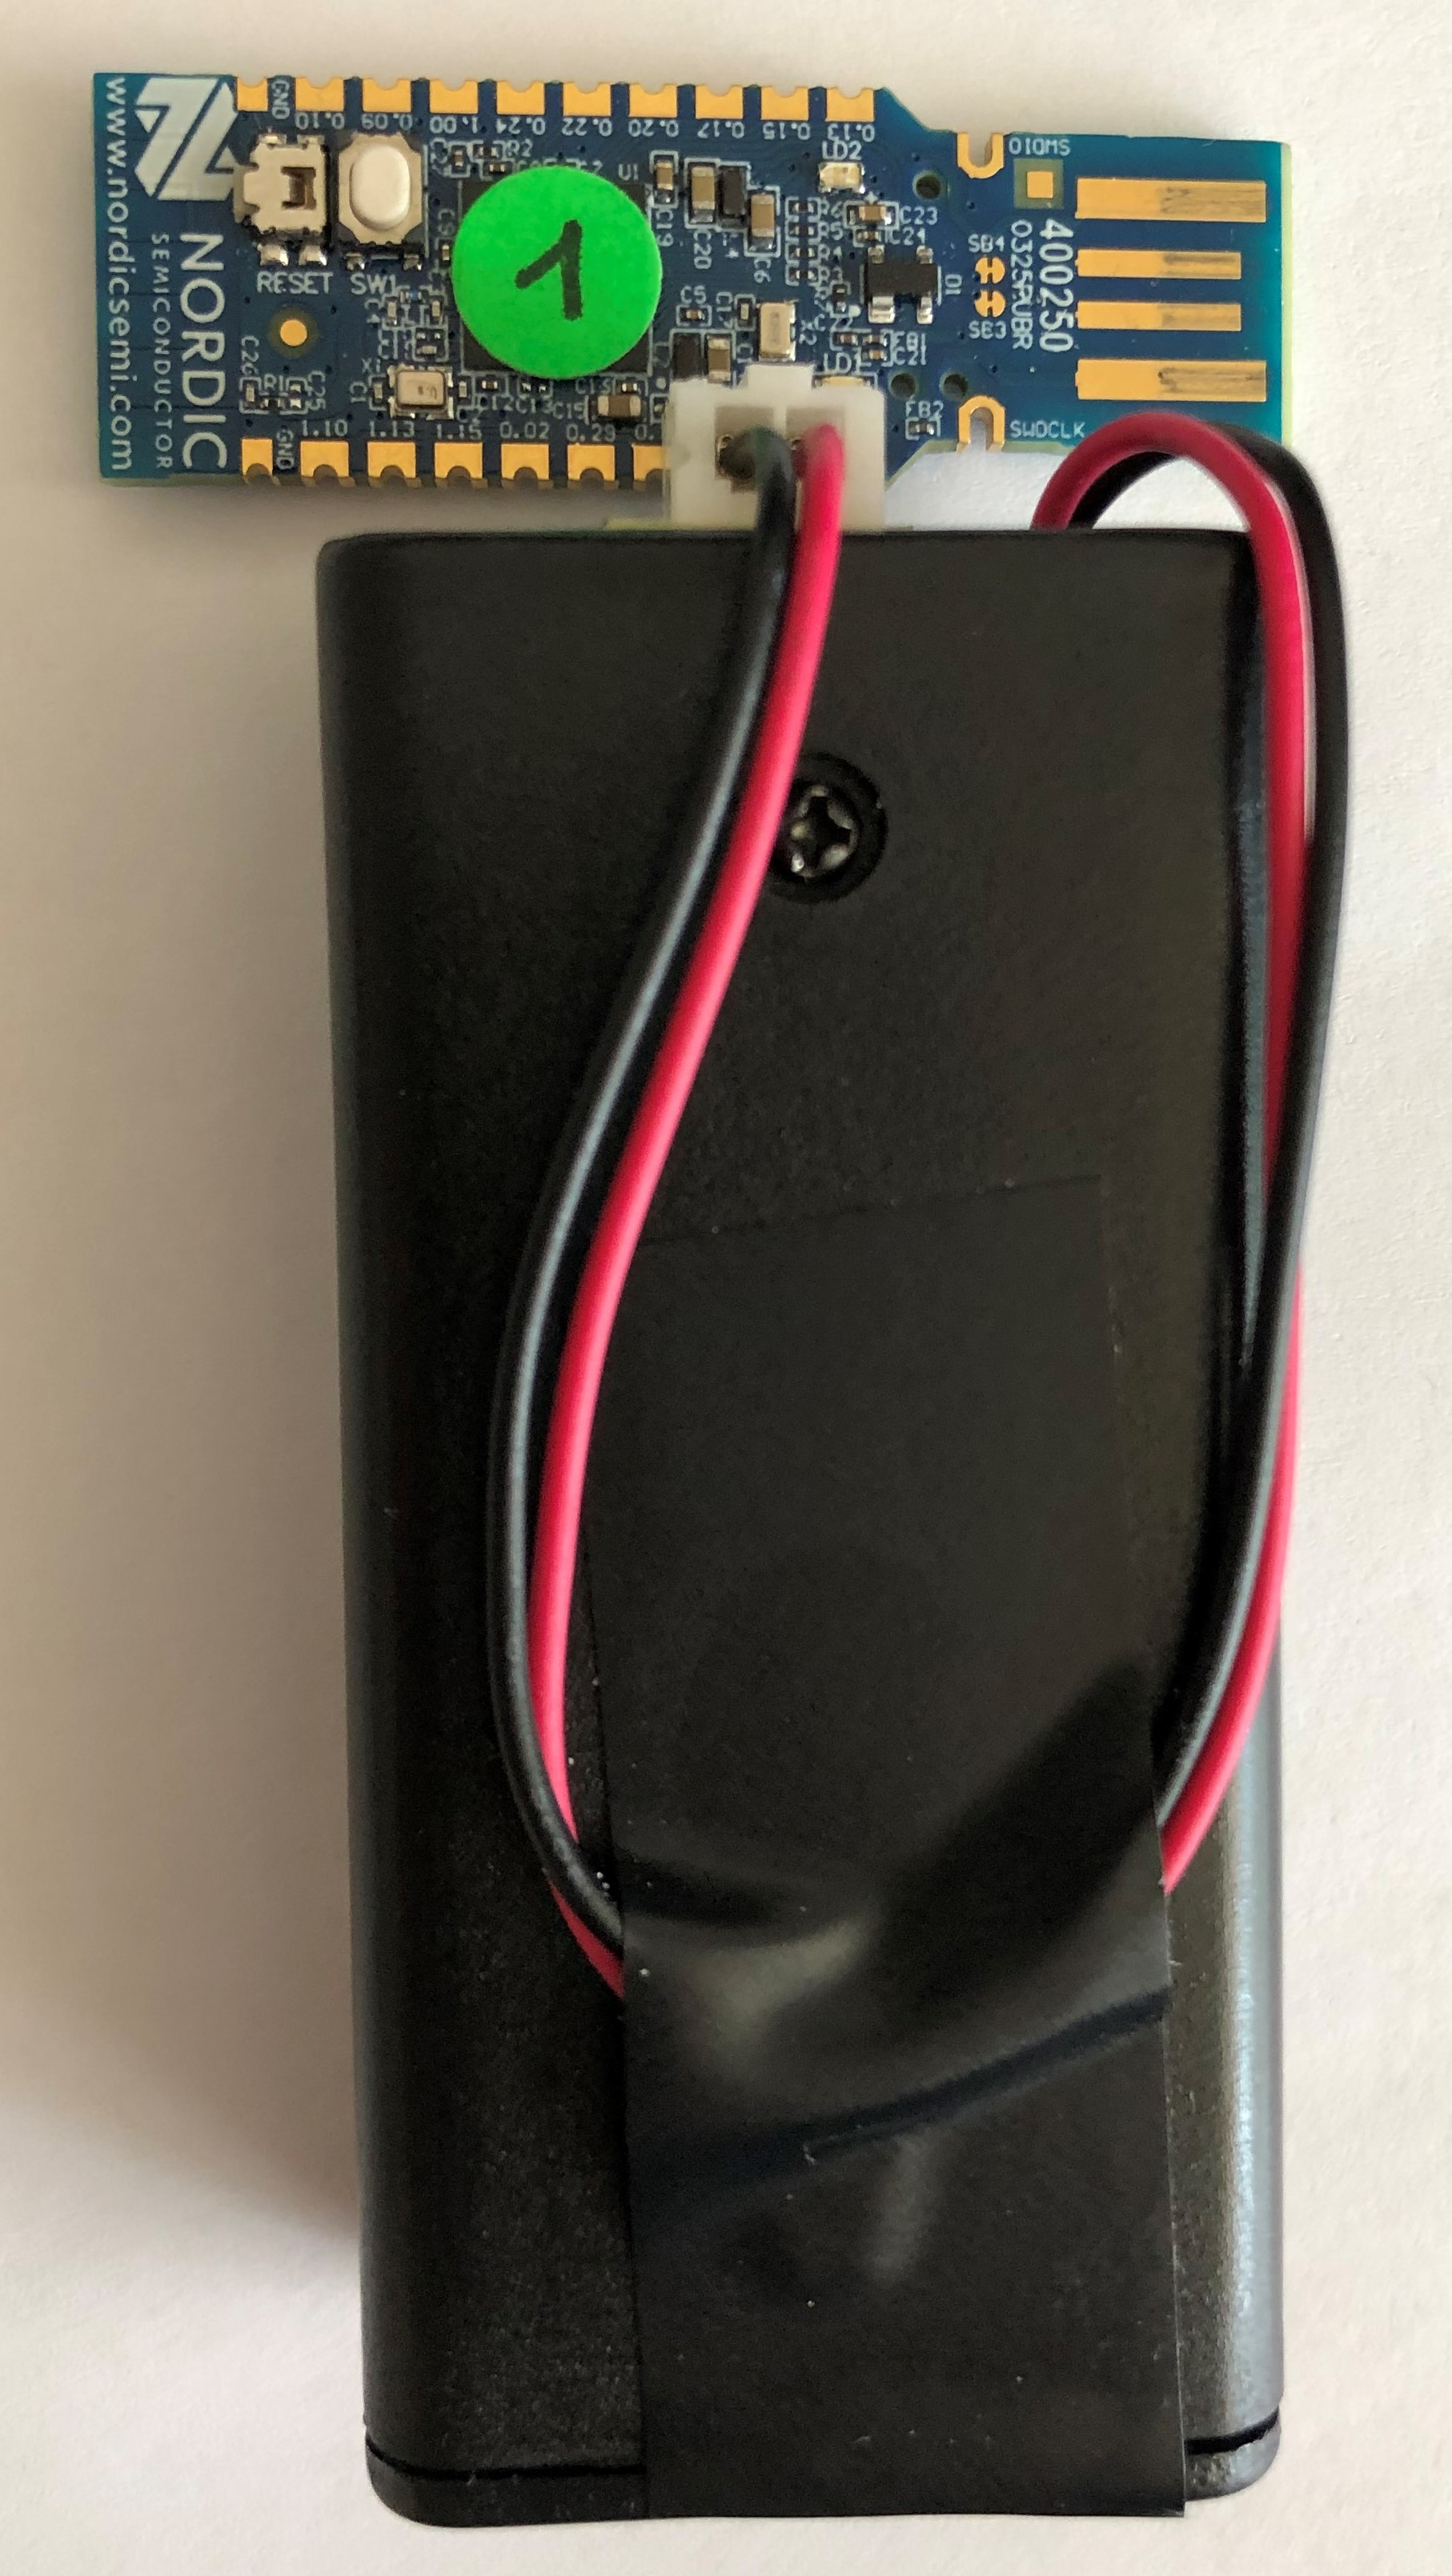
\includegraphics[width=0.4\columnwidth]{graphics/Node_picture.png}
    \end{center}

    \newcol
    \section{Resultate}
}

\infobox{Erkenntnisse}{
	 \begin{minipage}{0.50\textwidth}
     \setlength\leftmargini{0.5em}
     \raggedright
     asödasdf asdlfkasd asdfölkasdf asdölfkasdf  asdfljasdfl 
     
    \end{minipage}
    \hfill
    \begin{minipage}{0.45\textwidth}
        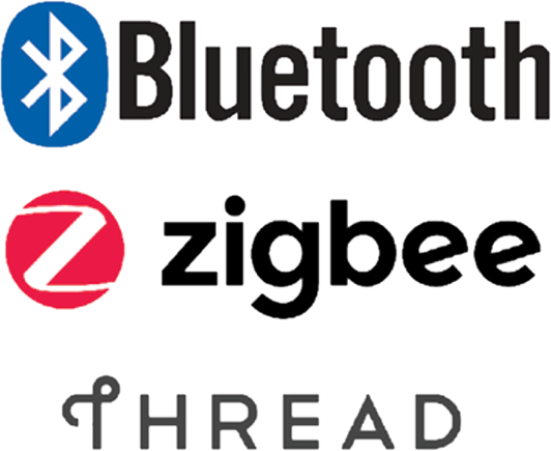
\includegraphics[width=\textwidth]{graphics/Protocols.png}
        \graphicssource{circuitcellar.com}
    \end{minipage}
}
